%=============================================================
% main.tex : IEEEtran + newtx + TikZ (English version)
%=============================================================
\documentclass[conference]{IEEEtran}

% ---- Packages ----
\usepackage{newtxtext,newtxmath}
\usepackage{amsmath,amssymb}
\usepackage{siunitx}
\usepackage{booktabs}
\usepackage{graphicx}
\usepackage{tikz}
\usetikzlibrary{arrows.meta, positioning, shapes}

%=============================================================
\begin{document}

\title{From JSON to ASIC: An Integrated $H_\infty$ Design Flow for Robust Spacecraft Control}

\author{\IEEEauthorblockN{Shinichi Samizo}
\IEEEauthorblockA{Independent Semiconductor Researcher\\
Project Design Hub / EduController\\
Email: shin3t72@gmail.com}}

\maketitle

%=============================================================
\begin{abstract}
We present an end-to-end $H_\infty$ control design flow for spacecraft autonomy,
starting from JSON descriptions of plant and weighting functions, and reaching
a radiation-hardened 22FDX ASIC implementation. The workflow integrates
EduController for model generation, AITL-H for $H_\infty$ synthesis, fixed-point
realization, RTL translation, FPGA hardware-in-the-loop (HIL) verification,
and FEM-based closure with thermal and radiation conditions. This unifies
control synthesis and VLSI implementation, minimizing gaps between theory and
deployment in long-duration space missions.
\end{abstract}

%=============================================================
\section{Introduction}
Spacecraft autonomy demands robust control architectures that can survive
total ionizing dose (TID), single-event effects (SEE), and long-term thermal
cycling. Traditional PID + Flash architectures face reliability bottlenecks.
To address these issues, we propose a design flow that tightly couples control
theory with implementation, ensuring that $H_\infty$ controllers derived at
the system level are carried forward seamlessly to ASIC tape-out.

%=============================================================
\section{Design Flow Overview}
EduController exports the plant dynamics and weighting functions in JSON
format. The AITL-H module consumes this data and synthesizes an
output-feedback gain $K$ by solving Riccati or LMI formulations of the
$H_\infty$ problem. The resulting controller is then quantized into fixed-point
representation, parameterized for RTL, and validated on FPGA HIL platforms
under injected radiation and sensor-fault scenarios.

%=============================================================
\section{From JSON to ASIC}
Fig.~\ref{fig:json-to-asic} illustrates the complete flow.

\begin{figure}[t]
\centering
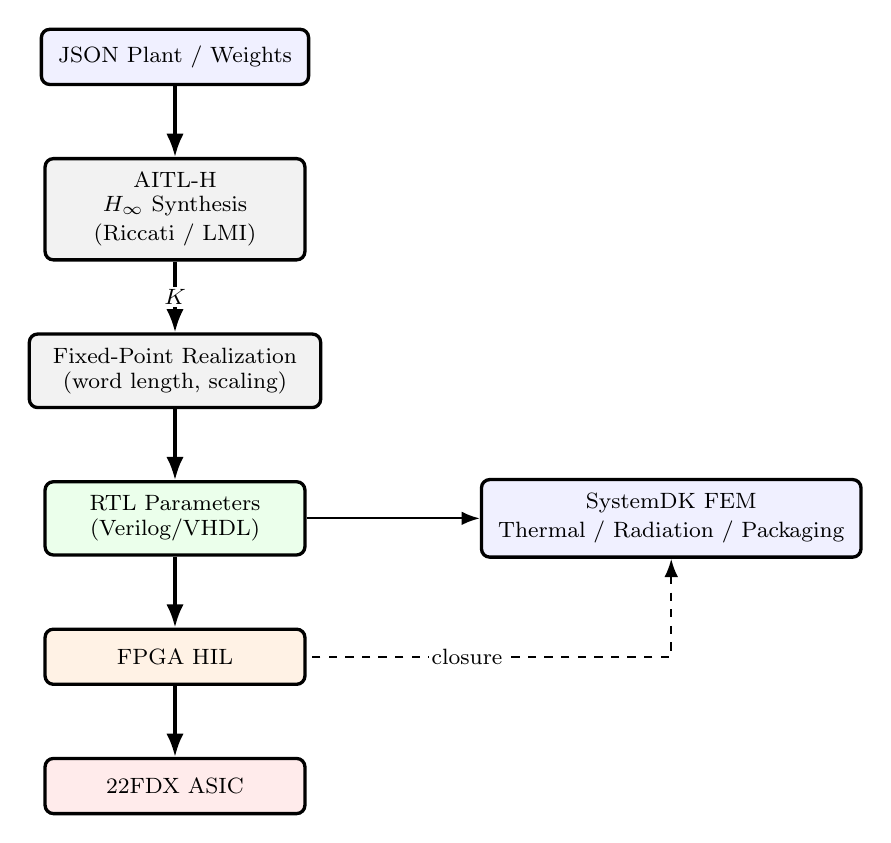
\begin{tikzpicture}[
  >=Latex,
  node distance=9mm and 15mm,
  font=\footnotesize,
  block/.style={
    draw, rounded corners=3pt, very thick,
    inner xsep=6pt, inner ysep=5pt,
    minimum width=33mm, minimum height=7mm,
    align=center
  },
  blu/.style={block, fill=blue!6},
  grn/.style={block, fill=green!8},
  org/.style={block, fill=orange!10},
  red/.style={block, fill=red!8},
  gry/.style={block, fill=gray!10},
  lab/.style={midway, fill=white, inner sep=1pt}
]

% --- Nodes (top→bottom main flow)
\node[blu] (json) {\shortstack{JSON Plant / Weights}};
\node[gry, below=of json] (hinf) {\shortstack{AITL-H \\ $H_\infty$ Synthesis\\(Riccati / LMI)}};
\node[gry, below=of hinf, minimum width=37mm] (fxp) {\shortstack{Fixed-Point Realization \\ (word length, scaling)}};
\node[grn, below=of fxp] (rtl) {\shortstack{RTL Parameters \\ (Verilog/VHDL)}};
\node[org, below=of rtl] (hil) {\shortstack{FPGA HIL}};
\node[red, below=of hil] (asic) {\shortstack{22FDX ASIC}};

% --- Side (FEM closure)
\node[blu, right=22mm of rtl, minimum width=42mm] (fem) {\shortstack{SystemDK FEM \\ Thermal / Radiation / Packaging}};

% --- Arrows main
\draw[->, very thick] (json) -- (hinf);
\draw[->, very thick] (hinf) -- node[lab] {$K$} (fxp);
\draw[->, very thick] (fxp) -- (rtl);
\draw[->, very thick] (rtl) -- (hil);
\draw[->, very thick] (hil) -- (asic);

% --- Arrows side
\draw[->, thick] (rtl.east) -- (fem.west);
\draw[<-, thick, dashed] (fem.south) |- node[lab, pos=0.78]{closure} (hil.east);

\end{tikzpicture}
\caption{End-to-end $H_\infty$ design flow ``from JSON to ASIC''. EduController
exports plant and weights in JSON; AITL-H synthesizes the controller gain $K$;
quantization and RTL mapping follow; FPGA HIL validates functionality; finally,
a 22FDX ASIC is taped out. SystemDK FEM provides closure with thermal and
radiation scenarios.}
\label{fig:json-to-asic}
\end{figure}

%=============================================================
\section{Conclusion}
This paper outlined a unified workflow that bridges $H_\infty$ control
synthesis with VLSI implementation. Starting from JSON-based models, the flow
carries the design through synthesis, quantization, RTL, FPGA HIL, and ASIC
integration, while closing the loop with FEM verification. This approach
provides a practical route toward resilient autonomy in deep-space missions.

%=============================================================
\bibliographystyle{IEEEtran}
\begin{thebibliography}{1}
\bibitem{Doyle}
J. C. Doyle, B. A. Francis, and A. R. Tannenbaum, \textit{Feedback Control Theory}. Macmillan, 1992.
\bibitem{Colinge}
J.-P. Colinge, \textit{Silicon-on-Insulator Technology: Materials to VLSI}, 3rd ed. Springer, 2004.
\end{thebibliography}

\end{document}
